\question[5]
\begin{minipage}[]{.45\linewidth}
Gegeben sei das nebenan abgebildete Szenario. Der Client möchte eine HTTP-Anfrage
an den Web Server stellen, kennt aber nur dessen symbolischen Namen. Deshalb
muss zunächst eine DNS-Anfrage erfolgen. Es wird angenommen, dass die Caches
der DNS-Server und des Clients leer sind.  Berücksichtigen Sie für die folgenden
Berechnungen ausschließlich die RTTs, keine anderen Verzögerungen.

Wie lange dauert eine DNS Anfrage des Clients, welche \VAR{rekit} erfolgt?
\end{minipage}
\hfill
\begin{minipage}[]{.45\linewidth}
	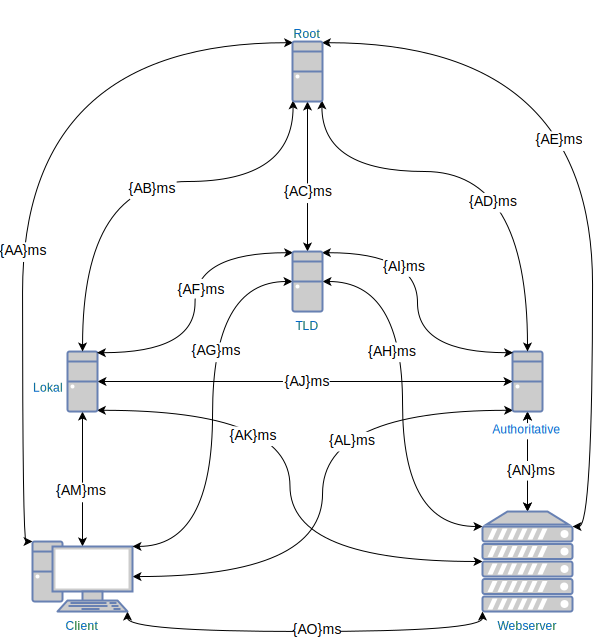
\includegraphics[width=\linewidth]{DNS_Hierarchie.png}
\end{minipage}


\begin{solutionbox}{1.5cm}
	%- if rekit == 'rekursiv':
	\[\VAR{AM}ms + \VAR{AB}ms + \VAR{AC}ms + \VAR{AI}ms = \VAR{AM + AB + AC + AI}ms\]
	%- else
	\[\VAR{AM}ms + \VAR{AB}ms + \VAR{AF}ms + \VAR{AJ}ms = \VAR{AM + AB + AF + AJ}ms\]
	%- endif
\end{solutionbox}
